\documentclass[12pt, twoside]{article}
\usepackage[letterpaper, margin=1in, headsep=0.5in]{geometry}
\usepackage[english]{babel}
\usepackage[utf8]{inputenc}
\usepackage{amsmath}
\usepackage{amsfonts}
\usepackage{amssymb}
\usepackage{tikz}
\usetikzlibrary{quotes, angles}
\usepackage{graphicx}
\usepackage{enumitem}
\usepackage{multicol}
\usepackage{hyperref}

\newif\ifmeta
\metatrue %print standards and topics tags

\title{IB Mathematics}
\author{Chris Huson}
\date{February 2022}

\usepackage{fancyhdr}
\pagestyle{fancy}
\fancyhf{}
\renewcommand{\headrulewidth}{0pt} % disable the underline of the header
\raggedbottom


\fancyhead[LE]{\thepage}
\fancyhead[RO]{\thepage \\ Name: \hspace{4cm} \,\\}
\fancyhead[LO]{BECA / IB Math 5 Exponential functions \\* 16 February 2022}

\begin{document}

\subsubsection*{5.3 Classwork: Exponential function bases}
I can calculate simple interest \hfill CCSS.HSF.IF.C.7

\begin{enumerate}
\item Do Now: Carlos puts \$12,500 into an investment account with an annual interest rate of 3.15\%. What is the balance after 5 years? \vspace{2cm}

\item The graph shows the exponential function $\displaystyle f(x)=1000 \times \left( 1.25 \right)^t$ representing growth with a base of 1.25 over $t$ periods.
\begin{multicols}{2}
    \begin{enumerate}[itemsep=1cm]
        \item Write down the initial value of the function.
        \item Find $f(10)$
        \item Find $x$ such that $y=6000$
    \end{enumerate}
    \begin{center}
    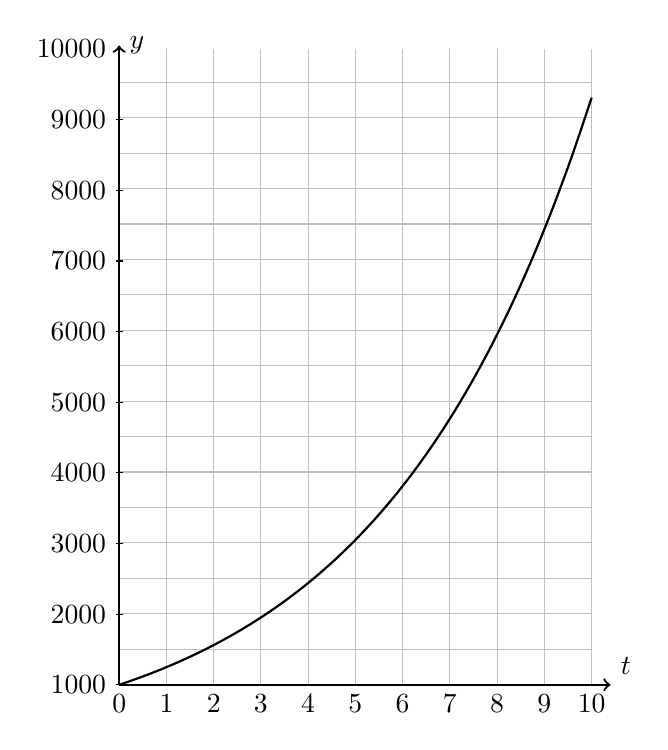
\begin{tikzpicture}[x=1cm, y=0.0015cm, scale=0.6]
        \draw [thin, color=lightgray, xstep=1.0cm,ystep=0.75cm] (0,1000) grid (10,10000);
        \draw [thick, ->] (0,1000) -- (+10.4,1000) node [above right]{$t$};
        \draw [thick, ->] (0,1000) -- (0,10050) node [right]{$y$};        \foreach \x in {0,1,...,10}
            \draw (\x cm,1000) -- (\x cm,1000) node[below] {$\x$};
        \foreach \y in {1000,2000,...,10000}
            \draw[shift={(0,\y)}] (2pt,0pt)--(-2pt,0pt) node[left]{$\y$};
        
        \draw [thick, smooth,domain=0.:10] plot(\x,{1000*(1.25^\x)});
    \end{tikzpicture}
    \end{center}
    \end{multicols}

\item Radioactive elements decay over time, with one half of the atoms decaying over a fixed period of time, the ``half life.'' The half life of plutonium-238 is about 90 years. Use the formula $\displaystyle y=A \times \left( \frac{1}{2} \right)^{t/90}$. 
\begin{enumerate}[itemsep=1.5cm]
    \item Find the percentage of plutonium that would remain after 1000 years.
    \item Find the number of years required for 99 percent of the plutonium to decay.
\end{enumerate}

\newpage
\subsubsection*{5.3 Exit Note: Simple interest rates}
\item Simplify each expression to the base raised to a power.
    \begin{multicols}{2}
    \begin{enumerate}[itemsep=0.5cm]
        \item $7^3 \times 7^6$
        \item $\displaystyle \frac{5^8}{5^4}$
        \item $x^2 \times x^9$
        \item $\displaystyle \left( \frac{z^7}{z^2}\right)^{2}$
    \end{enumerate}
    \end{multicols}

\item A bank account earns interest at an annual interest rate of 5.125\%. The initial deposit is \$225. Which equation models the value of the balance?
\begin{multicols}{2}
    \begin{enumerate}[itemsep=0.5cm]
        \item $\displaystyle FV=225 \cdot \left( \frac{5.125}{100}\right)^{t}$
        \item $FV=225 (1+5.125)^{t}$
        \item $FV=225 \cdot 5.125^{t}$
        \item $\displaystyle FV=225 \cdot \left(1+ \frac{5.125}{100}\right)^{t}$
    \end{enumerate}
\end{multicols}

\item Carlos puts \$9,800 into an investment account with an annual interest rate of 2.75\%. What is the balance after 3 years, rounded to the nearest cent? \vspace{2cm}

\item The graph shows the exponential function $\displaystyle FV=1,100 \times \left( 1+\frac{6.125}{100} \right)^t$ representing the balance of an investment account earning a fixed rate of interest over $t$ in years.
\begin{multicols}{2}
    \begin{enumerate}[itemsep=1cm]
        \item Write down the initial deposit in the account.
        \item What is the annual interest rate?
        \item Approximately how much will the account hold at the end of ten years?
        \item When will the balance be \$1,400?
    \end{enumerate}
    \begin{center}
    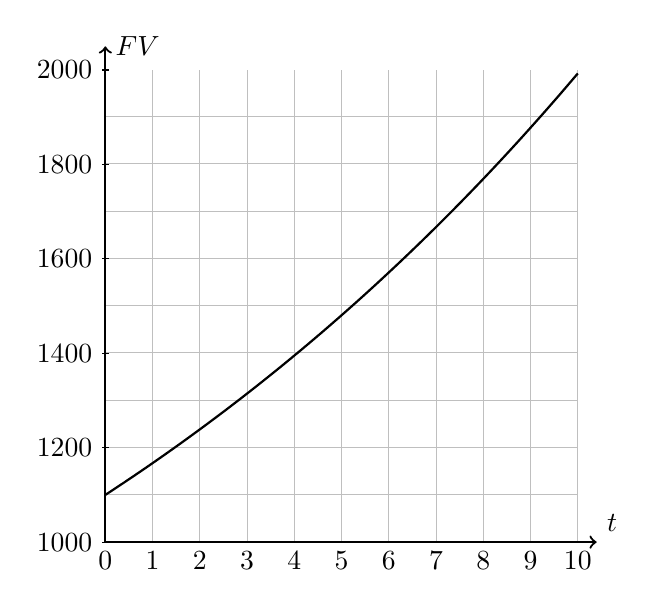
\begin{tikzpicture}[x=1cm, y=0.01cm, scale=0.6]
        \draw [thin, color=lightgray, xstep=1.0cm,ystep=1.0cm] (0,1000) grid (10,2000);
        \draw [thick, ->] (0,1000) -- (+10.4,1000) node [above right]{$t$};
        \draw [thick, ->] (0,1000) -- (0,2050) node [right]{$FV$};        \foreach \x in {0,1,...,10}
            \draw (\x cm,1000) -- (\x cm,1000) node[below] {$\x$};
        \foreach \y in {1000,1200,...,2000}
            \draw[shift={(0,\y)}] (2pt,0pt)--(-2pt,0pt) node[left]{$\y$};

        \draw [thick, smooth,domain=0.:10] plot(\x,{1100*(1.06125^\x)});
    \end{tikzpicture}
    \end{center}
    \end{multicols}

\end{enumerate}
\end{document}



